
\documentclass[tikz,border=2pt]{standalone}
\usepackage{amsmath,amssymb}
\usepackage{amsfonts}
\usepackage{xcolor}
\usetikzlibrary{arrows.meta,positioning,calc,shapes,decorations.pathreplacing}
% Define some common colors used in IR lectures if any
\definecolor{sparse}{rgb}{0.8,0.8,1}
\definecolor{dense}{rgb}{1,0.8,0.8}
\begin{document}
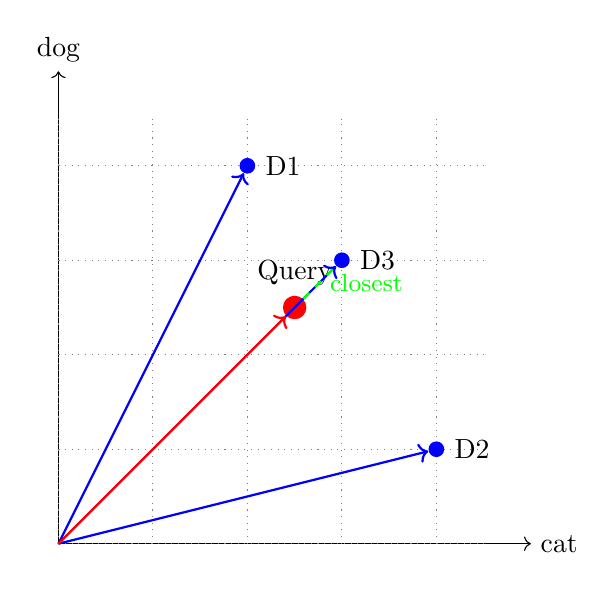
\begin{tikzpicture}[scale=1.2]
    
    \draw[->] (0,0) -- (5,0) node[right] {cat};
    \draw[->] (0,0) -- (0,5) node[above] {dog};
    
    
    \draw[gray, dotted] (0,0) grid (4.5,4.5);
    
    
    \node[circle, fill=blue, inner sep=2pt, label=right:D1] (d1) at (2,4) {};
    \node[circle, fill=blue, inner sep=2pt, label=right:D2] (d2) at (4,1) {};
    \node[circle, fill=blue, inner sep=2pt, label=right:D3] (d3) at (3,3) {};
    
    
    \node[circle, fill=red, inner sep=3pt, label=above:Query] (q) at (2.5,2.5) {};
    
    
    \draw[->, thick, blue] (0,0) -- (d1);
    \draw[->, thick, blue] (0,0) -- (d2);
    \draw[->, thick, blue] (0,0) -- (d3);
    \draw[->, thick, red] (0,0) -- (q);
    
    
    \draw[dashed, green, thick] (q) -- (d3) node[midway, right] {\small closest};
\end{tikzpicture}
\end{document}
